\chapter{Architectural Design}\label{c:arch}

\section{Overview}

At the highest level of abstraction, the architecture of Data4Help and AutomatedSOS system is a common three-tier client/server paradigm, as shown in Figure \ref{f:3tier}.





\begin{figure}[H]
\centering
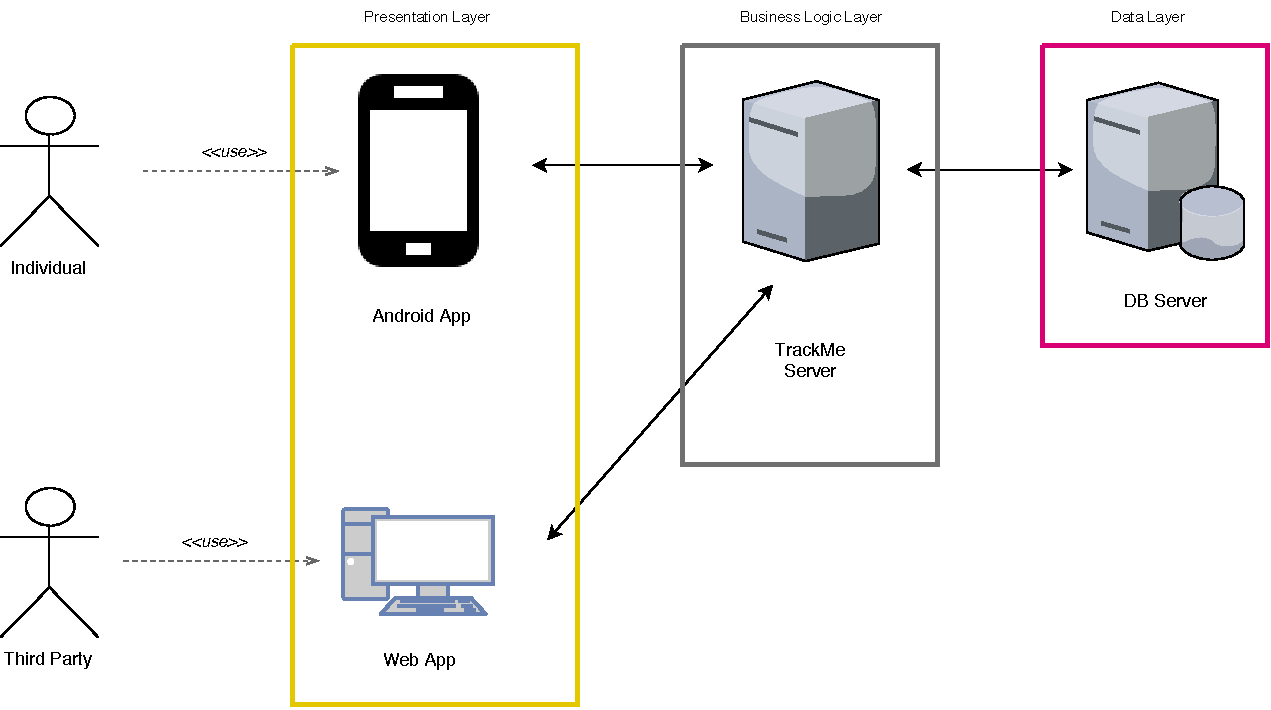
\includegraphics[scale=0.65]{resources/overview}
\caption{The 3 tier architecture of the system}\label{f:3tier}
\end{figure}
\noindent
The three layers are the following:

\begin{itemize}
\item \textbf{Presentation layer}: this layer is hosted on the users' devices, that are the smartphone for the individuals and a computer with a browser for third parties.
The GUIs are deployed in this layer.
\item \textbf{Business logic layer}: this layer contains the main components of the systems that carry out the operations needed for Data4Help and AutomatedSOS services.
\item \textbf{Data layer}: this layer is responsible for managing all the data of the system. 
In particular, it stores the data on persistent devices and makes them available when requested by the TrackMe server.
\end{itemize}
The structure displayed in Figure \ref{f:3tier} is not to be understood as a rigid constraint on the implementation choices, but it represents where most of the three three logic layers are deployed.
For examples, it is possible that part of the data is (temporarily) stored on the clients in order to reduce latency or that some presentation logic is deployed on the TrackMe Server in order to achieve a more dynamic GUI.





\section{Component view}
The diagram in Figure \ref{f:comp_diag} examines in more detail the subcomponents composing the TrackMe server.
Some components requires external services, this is shown by means of pending required interfaces.
All the four components defined below have access to the database server interface in order to store and retrieve the data necessary for their correct operation.

\begin{figure}[H]
\centering
\includegraphics[width=\linewidth]{resources/uml/compdiag}
\caption{Component Diagram}\label{f:comp_diag}
\end{figure}

\noindent
As shown, there are four main components in the business logic server:

\begin{itemize}
\item \textit{Login Manager}: is responsible for the login and registration of the users, both individuals and third parties.
\item \textit{Data Collector}: is responsible of collecting data from the Android App. 
It also forwards the proper data to the Automated SOS component.

\item \textit{Data Manager}: receives and handles requests from third parties and push to them new data when available and the subscription is valid.
For certain functionalities, for example for geographically filter the data, the Data Manager component requires an external API to a map service.
It also makes possible for the individuals to visualize their data.

\item \textit{Automated SOS}: handles the subscriptions for the SOS service. 
Every time that it receives new data from the Data Collector, the component checks whether the thresholds are crossed, in this case it immediately calls an ambulance through an external API.
\end{itemize}
In addition, Figure \ref{f:comp_diag} shows that the Android App component requires an interface towards the wearable device, from which it will gather the eHealth Data.




\section{Deployment view}



The diagram in Figure \ref{f:depl_diag} shows the physical deployment of system's artifacts on various nodes.
In particular, the nodes are:

\begin{itemize}
\item \textit{Smartphone}: this device is used by an individual, then the Android Application is deployed here. This node interacts with the Business Server.
\item \textit{Personal Computer}: this device is used by a third party, only a modern browser compatible with HTML5 and CSS3 is required. Actually, there are no artifacts of our system deployed on this node, because the interaction is carried out with a Web App directly towards the Business Server.
\item \textit{Business Server}: this is the core node of our system.
All the Business Logic is deployed here, possibly by means of an Application Server like GlassFish.
This is the only node that interact with the Database node.
\item \textit{Data Server}: on this node are deployed all the artifacts necessary to manage the data.
\end{itemize}


\begin{figure}[h]
\centering
\includegraphics[width=\linewidth]{resources/uml/depldiag}
\caption{Deployment Diagram}\label{f:depl_diag}
\end{figure}

\section{Component Interfaces}
The following diagram shows what features each component must provide to guarantee the correct functioning of Data4Help features, highlighting the dependencies among the various components.
To make the diagram more clear, the crossing arrows have different colors and the external components are highlighted in orange.
Following the diagram, each operation is defined through a brief description.

\begin{figure}[H]
\centering
\includegraphics[width=\linewidth]{resources/uml/Interfacediag}
\caption{Interface Diagram}\label{f:inter_diag}
\end{figure}


\begin{itemize}
\item Android App
\begin{itemize}
\item \textbf{forwardAccessRequest}: forwards the third party data access request to the individual's application. The data request is taken as an input parameter because it is needed to retrieve all the information about the request: who is the requester, in which data he is interested in.
\end{itemize}
\item Wearable Service
\begin{itemize}
\item \textbf{downloadData}: downloads the data stored in the paired wearable.
\item \textbf{checkVitalSensors}: checks if the wearable is capable of measuring at least one vital parameter, either the blood pressure or the heart rate.
\end{itemize}
\item Web App
\begin{itemize}
\item \textbf{notifyEndSubscription}: sends a notification to the Web App about the ended subscription of the data request passed as an input parameter.
\item \textbf{sendData}: sends the given data to the Web App.
\end{itemize}
\item Data Collector
\begin{itemize}
\item \textbf{sendData}: sends the gathered data from the Android App to the Data Collector.
\end{itemize}
\item Map Service
\begin{itemize}
\item \textbf{getMapCoordinates}: searches the coordinates of the border associated to the given map zone. These coordinates will be then used by the DBMS in order to apply filters to the stored data based on geographical zones.
\end{itemize}
\item Data Manager
\begin{itemize}
\item \textbf{checkGroupCostraints}: operation used to check if the group data found by the database applying the data request filters specified by the third party counts at least 1001 individuals.
\item \textbf{giveAccess}: allows the individual data gathering from the given third party request to be processed.
\item \textbf{denyAccess}: denies the individual data gathering from the given third party request to be processed.
\item \textbf{subscribeData}: activates the data subscription for the given data request.
\end{itemize}
\item Login Manager
\begin{itemize}
\item \textbf{createAccount}: uses the given credentials to create a Data4Help account.
\item \textbf{logIn}: allows users to access to Data4Help through their username (or tax code in case it is an individual) and password digest.
\end{itemize}
\item Automated SOS
\begin{itemize}
\item \textbf{subscribe}: activates the AutomatedSOS service for the individual associated to the given tax code.
\item \textbf{unsubscribe}: stops the AutomatedSOS for the individual associated to the given tax code.
\item \textbf{checkVitalThresholds}: checks if the data of the vital paramaters have crossed the critical thresholds
\end{itemize}
\item Ambulance Service
\begin{itemize}
\item \textbf{callAmbulance}: calls an ambulance, using the input coordinates to specify the destination.
\end{itemize}
\item DBMS
\begin{itemize}
\item \textbf{addSubscriber}: promotes the individual account associated to the given tax code as an AutomatedSOS account.
\item \textbf{removeSubscriber}: removes the AutomatedSOS subscription from the account bound to the tax code.
\item \textbf{getData}: uses the given data filters to retrieve the desired data.
\item \textbf{uploadData}: adds the given data to the database.
\item \textbf{retrieveAccount}: checks if the given credentials are in the database.
\item \textbf{createAccount}: adds a new user account to the database using the given credentials.
\item \textbf{getDuplicate}: retrieves a tuple matching the given username or tax code.
\item \textbf{updateAccess}: updates the list of all third parties that can have access to the individual data.
\item \textbf{getAccessibleIndividual}: finds the tuple containing the given third party username and individual identifier, from the table containing all the list of the third parties and the individuals of which they have data access.
\item \textbf{getNewData}: collects all the new data related to a data request.
\item \textbf{getIndividual}: retrieve the given individual from the DB.
\end{itemize}
\end{itemize}
Note that the operations associated to the external services are fictitious, the real names or input parameters may vary from the one listed above, but the expected functionalities must be the same, even if they are mapped on more than one real function.\\
In particulare the DBMS operations are just queries to the DB.

In this document the model of the application will not be provided: this makes the development phase more flexible.\\
However, to better coordinate the interactions between the component, a general description of the input provided in each operation listed before is here presented:
\begin{itemize}
\item requiredCredentials: this will be a data structure containing multiple strings such as the taxCode, the username or the passwordDigest.
\item userIdentifier: this is a generic string that could be either the individual username or tax code, or the third party username.
\item individualIdentifier: this generic string that could be either the individual username or tax code.
\item dataRequest: this will be the data structure that represents the data request from the third parties. It will contain all the filters applied for the data request, an Id a typology identifier for the request itself and the sender username.
\item mapAreas: list of strings representing the geographical filter applied by the third party.
\item dataFilters: this data structure contains all the filters that can be extrapolated from the dataRequest.
\item retrievedData: data structure containing all the data retrieved from the DB.
\item gatheredData: data structure containing all the data downloaded from the individual's smartwatch.
\item vitalParameterData: data structure containing all the individual data that is needed for the AutomatedSOS service.
\end{itemize}




\section{Runtime view}
The following diagrams shows the interactions between the interface components defined in the previous section in  order to provide Data4Help functionalities. Remember that, since Data4Help is a three-tier application based on a client/server architecture it is fundamental that the user applications and the server are connected to the internet.
\subsection{User registration}
\begin{figure}[H]
\centering
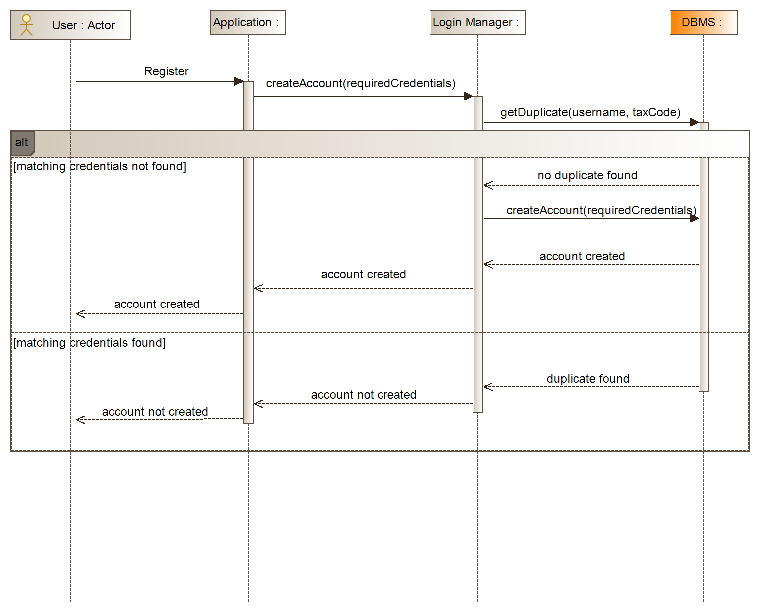
\includegraphics[width=\linewidth]{resources/uml/sequence/Registration.png}
\end{figure}
This diagram shows the procedure activated when the user registers to Data4Help.\\
The precondition of the registration is that the user has filled all the mandatory fields of the Sign Up form.\\
When the user presses the register button, the content of the compiled fields is sent to the Login Manager component to create an account.\\
Before creating the account, the LoginService checks through the DBMS services if the provided username and tax code are already present in the DB.\\
If the provided username or tax code is already taken, the procedure terminates sending an error notification to the client, otherwise the Login Manager adds the new account credentials in the DB through the DBMS.\\
After the account is created a notification is sent to the user and the procedure ends.


\subsection{User log in}
\begin{figure}[H]
\centering
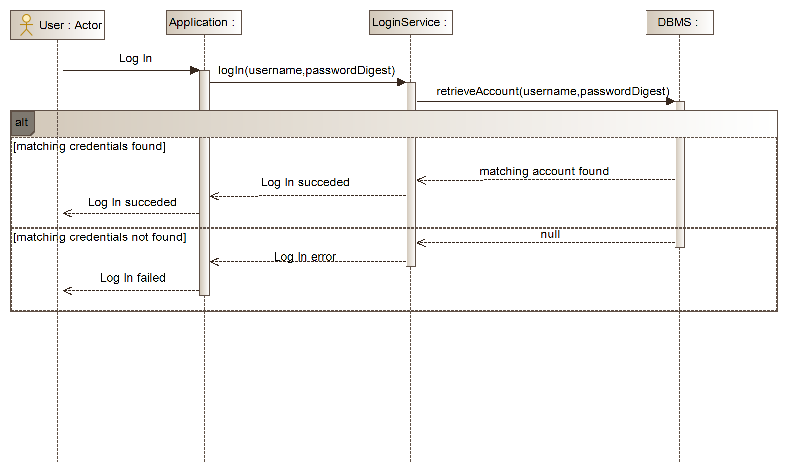
\includegraphics[width=\linewidth]{resources/uml/sequence/LogIn.png}
\end{figure}
In this diagram it's presented the Log In procedure.\\
Once the user has pressed the Log In button, the username and the password digest are sent to the Login Manager.\\
This component checks through the DBMS if there exists an account matching the credentials provided: in the positive case the user is logged in and directed to the respective data visualization screen, otherwise an error notification is sent to the user.\\
Notice that, in order to maintain user privacy the password is encrypted immediately with an hash function, and only its digest is used during this procedure.


\subsection{Individual data upload}
\begin{figure}[H]
\centering
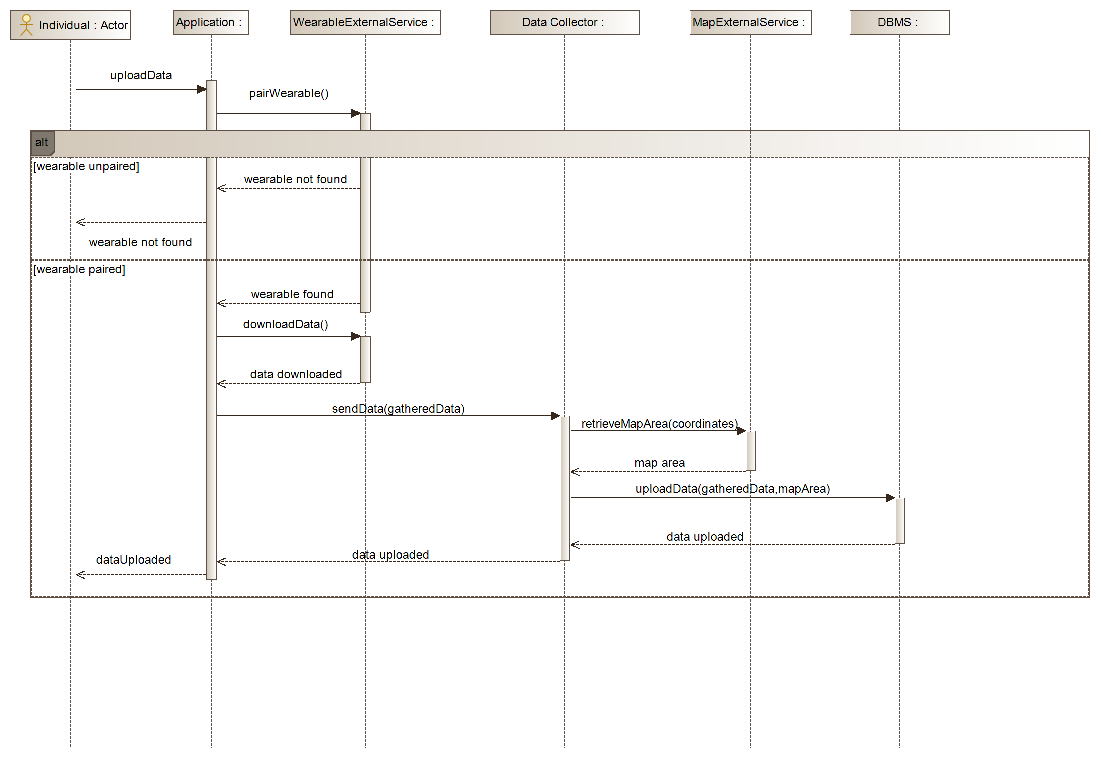
\includegraphics[width=\linewidth]{resources/uml/sequence/wearablePairing.png}
\end{figure}
This diagram shows the data upload procedure, including the wearable pairing phase.\\
Obviously the individual must be logged in, in order to start the data upload.\\
When the individual goes to the data visualization screen the wearable pairing, using the external wearable service, starts.\\
If the wearable is not found the procedure terminates sending an error notification to the application.
In the other case, once the wearable is paired, the application downloads the data gathered from the smartphone through the wearable services.\\
The downloaded data is then sent to the server through the Data Collector, that uploads the data into the DB through the DBMS.\\
Once the data is uploaded, a notification is sent to the Android App which now displays the new data.

\subsection{AutomatedSOS subscription}
\begin{figure}[H]
\centering
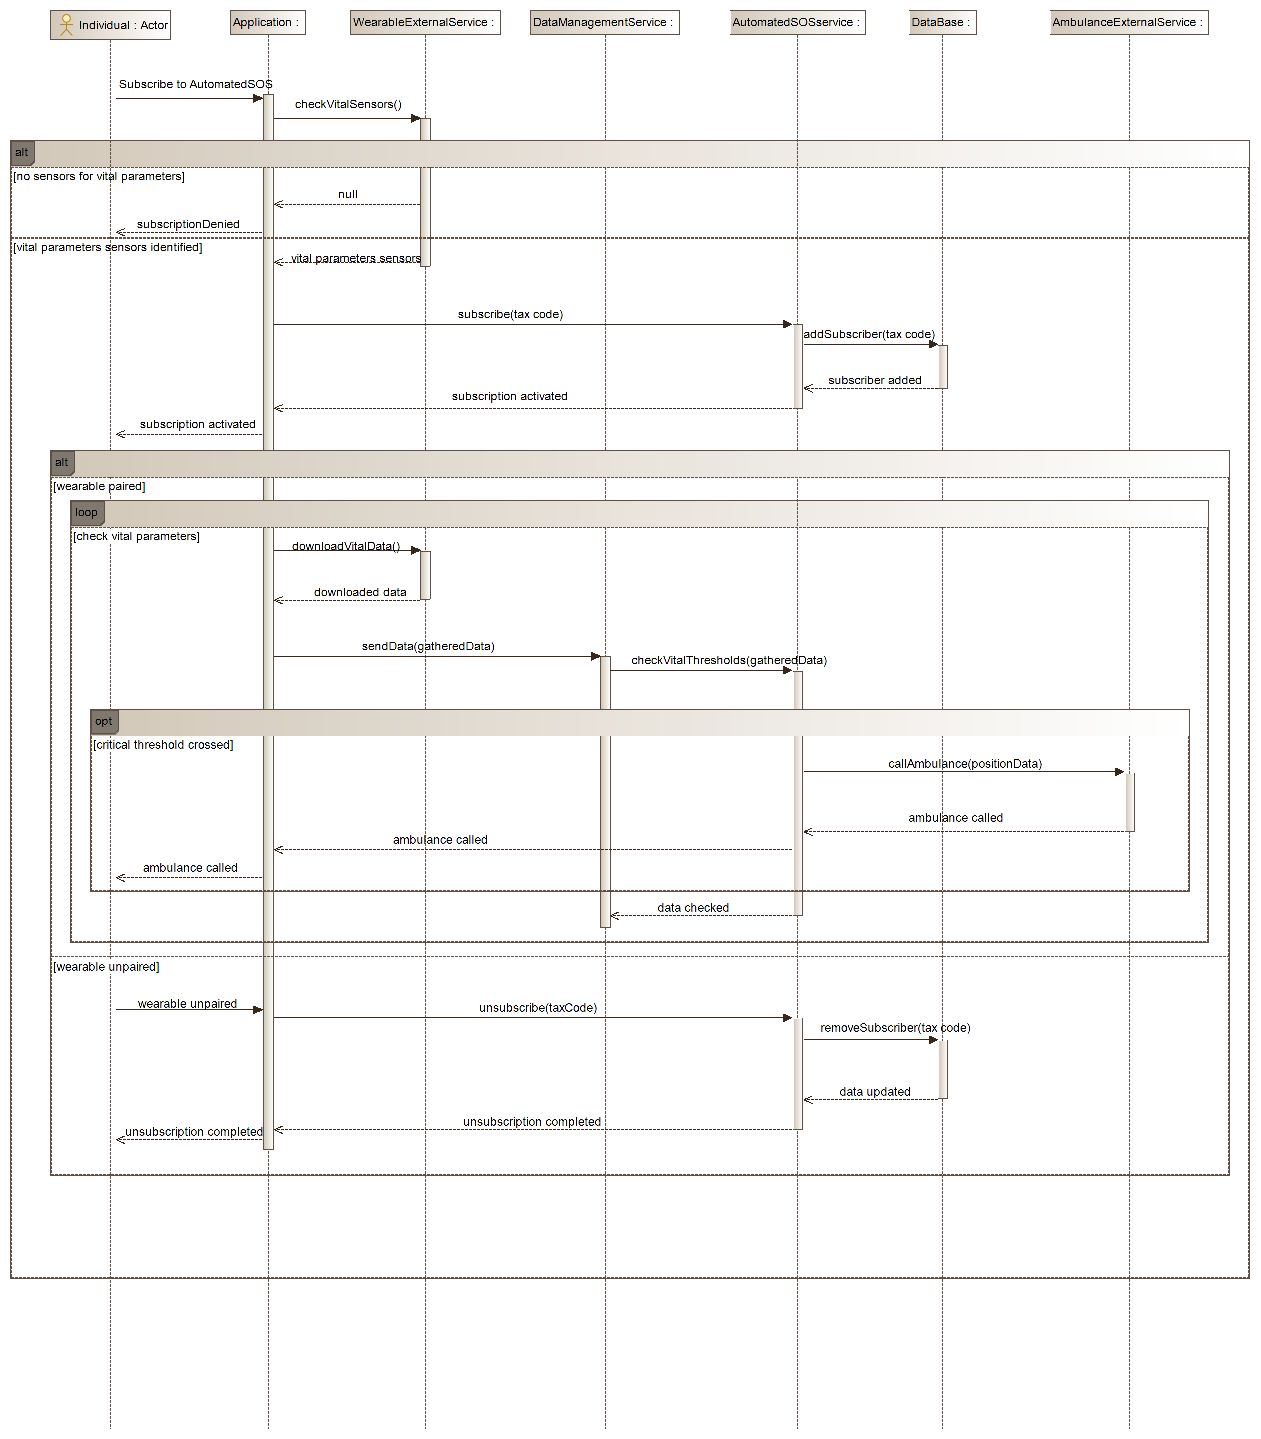
\includegraphics[width=\linewidth]{resources/uml/sequence/AutomatedSOS.png}
\end{figure}
This diagram illustrates the AutomatedSOS subscription procedure that is activated once the individual has paired the wearable and the subscribe button is tapped.\\
After the subscribe button is tapped, the application checks through the wearable external interface if the wearable is capable of measuring either the blood pressure or the heart rate.\\
In the negative case the procedure ends sending a notification to the individual.
In the other case, the application starts the subscription by using the Automated SOS component, that updates the DB setting the individual as an AutomatedSOS subscriber. Once the individual is set as a subscriber a notification is sent to the application, notifying the start of the service.\\
After the service is started, the application regularly downloads the vital parameter data using the wearable external service, enriches it with the individual position data and sends it to the data collector.\\
The data collector checks if the values of vital data collected have crossed the critical threshold using the Automated SOS component: if the critical threshold of a vital parameter is crossed this component calls an ambulance using the external Ambulance APIs, giving the coordinates to set the destination of the ambulance.\\
Once the ambulance is called a notification is sent to the user application.\\
The AutomatedSOS service is active as long as the wearable is paired: when the wearable unpairs the application starts the unsubscribe operation of the Automated SOS, which updates the DB by removing the subscription, and notify the user about the ended subscription.



\subsection{Group Data Request}
\begin{figure}[H]
\centering
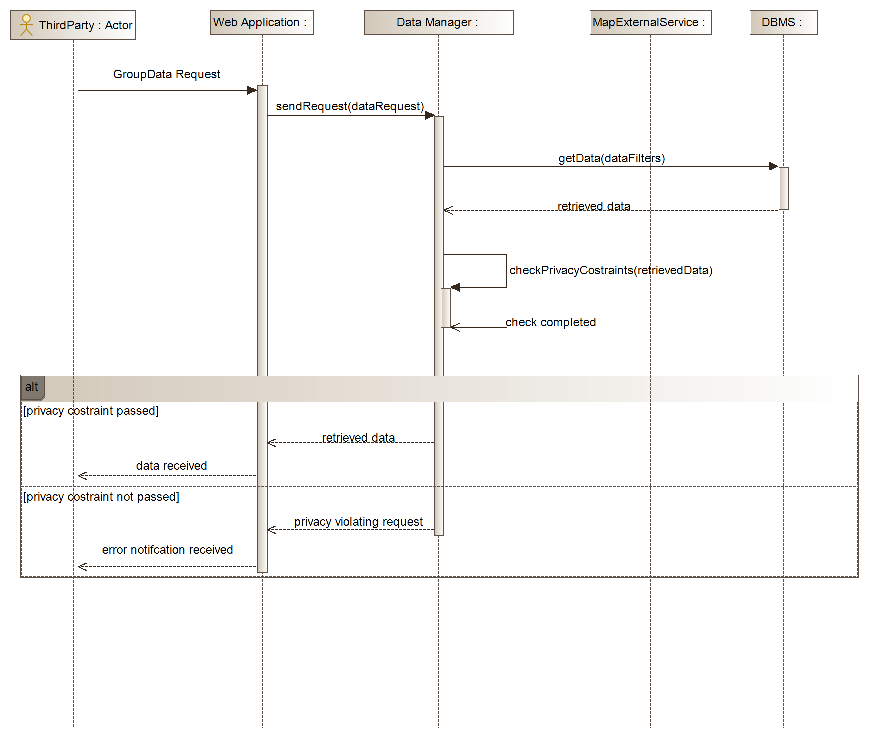
\includegraphics[width=\linewidth]{resources/uml/sequence/RequestGroupData.png}
\end{figure}
This diagram shows the interactions needed when a group data request from a third party occurs.\\
When a third party has filled the group data request form and clicks on the send button, the Web App sends the request to the Data Manager component.\\
This component retrieves the filters from the data request: if a geographical filter is applied, it uses the external map services to transform the given geographical filter in the corresponding border coordinates on the map.
Once the filters are retrieved it then uses the DMBS to gather the requested data.
Once the requested data is received, it checks if the privacy constraint is respected, by counting the number of individuals that are part of the selected data group: if it is above 1000 the data is forwarded to the WebApp, otherwise the request is denied and a notification is sent to the Web App.

\subsection{Individual Data request}
\begin{figure}[H]
\centering
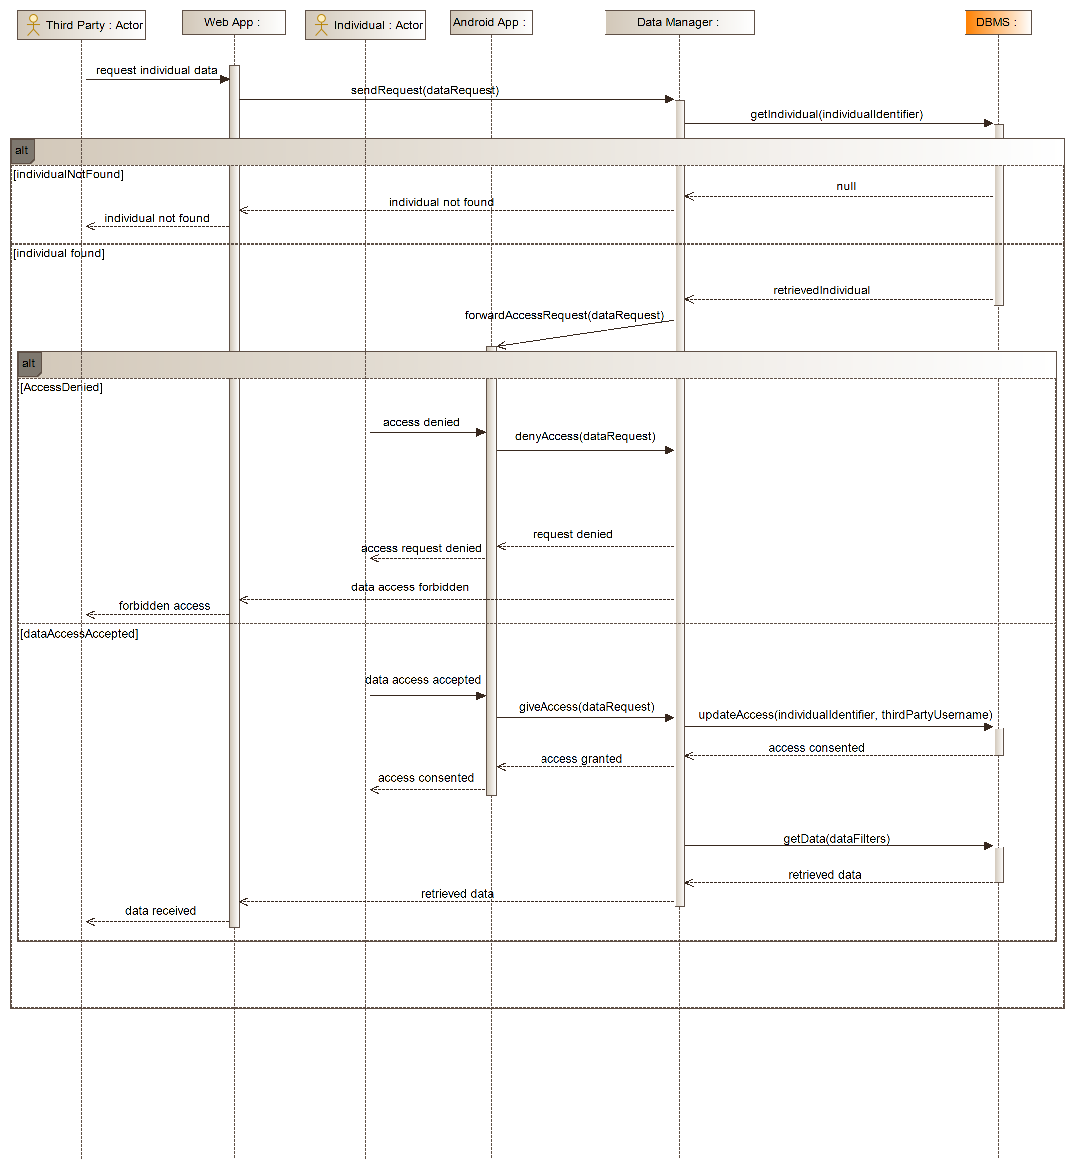
\includegraphics[width=\linewidth]{resources/uml/sequence/RequestIndividualData.png}
\end{figure}
In this diagram the individual data request is presented.\\
Similarly to what is done with the group data request, once the individual data request form is filled and the send button is clicked, the web application sends the request to the Data Manager component.\\
The first thing done by the Data Manager is to retrieve the individual requested from the DB: if he is not present a notification error is sent to the web application.\\
In the other case, the Data Manager forwards the access requests to the individual application.
The individual can choose to give the direct access of his data to the third party or deny it through the Android App: if the access request is refused the Android App notifies the Data Manager about the decision, which sends a notification to the third party.
If the individual allows the data access, the Data Manager sends the individual's data, retrieved through the DBMS, to the Web App.


\subsection{Group Data subscription}
\begin{figure}[H]
\centering
\includegraphics[width=\linewidth]{resources/uml/sequence/GroupDataSubscription.png}
\end{figure}
The above diagram shows the data subscription procedure that is activated when a third party decides to subscribe to a data request.\\
The Web App starts the subscription through the Data Manager component. Once the subscription is activated the Data Manager regularly checks if there is new data matching the data request to which the third party is subscribed to using the DBMS services.\\
If new data is found, the Data Manager checks if the privacy constraints are still active (both if the request is a group data request or an individual data request).\\
If the constraints are respected the new data is sent to the web application, otherwise the subscription is ended and the third party is notified about it.


\subsection{Individual Data subscription}
\begin{figure}[H]
\centering
\includegraphics[width=\linewidth]{resources/uml/sequence/IndividualDataSubscription.png}
\end{figure}
The individual data subscription procedure is very similar to the group one.\\
The only difference is that the regular check of the privacy constraint is done before retrieving the data, through the DBMS. Indeed, the DB contains the list of all the individuals whose data is accessible by each third party.\\ 


\section{Selected architectural styles and patterns}
\subsection{Overall Architecture}
Data4Help is based on a three tier architecture: almost all the system logic is executed in the server component, with the help of some external services.
The client applications mainly focus on presenting the information delivered by the server, however some functionalities may be delegated to it, for example the wearable pairing, which is handled by the individual application in order to give a faster response.
The data layer is handled by a single, well organized, DB. This choice was made to avoid data fragmentation among different databases.
\\

Moreover, the three tier architecture allows to make changes to any of the three layer without causing to much trouble to the other components: this is a fundamental aspect for system like Data4Help that continuously expands its functionalities.
\\

As stated in the RASD the availability is expected to be at 95\% of the annual time. Indeed there are no backup options in the system, all the component are in series with the server being the bottleneck due expected maintenance.\\
Obviously this value has to be improved over time, by acquiring new components to put in parallel to the old ones.

\subsection{Design Patterns}
The main design pattern used to build Data4Help is the ModelViewController design pattern.
This design pattern can be easily mapped to the client/server architecture used for Data4Help: the 
view part is obviously handled by the client applications, while the controller splits between the server and the client in order to pick the user input from the client and transform it into actions on the model stored in the server.
\\
The use of other design patterns, more related to the implementation, are left to the developers. 

\subsection{Other design decisions}
The main philosophy about the design process to Data4Help is to keep the system as simple as possible, since it offers few but well defined functionalities. This is useful to have a fast system, that can be developed quickly.\\
Furthermore, Data4Help strongly relies on external services:
\begin{itemize}
\item The Wearable external service is used to handle the pairing and the data download from the individual smartwatch. Initially the application will be build using Google wearOS APIs, but more smartwatches will be made compatible in the future.
\item The Map external service is used to translate the coordinates into geographical area names. Many options are available, and will be all considered in the development phase.
\item The Ambulance external service is used to call the ambulance. This services are provided by the local ambulance associations.
\end{itemize}


